
\section{background}
\label{sec:background}

Conflict-free Replicated Data Types belong to the optimistic
replication approach~\cite{saito2002replication,saito2005optimistic}. In the
context of distributed collaborative editing, the replicated data is a
document, where:
\begin{inparaenum}[(1)]
\item each insert/delete operation is prepared locally and broadcast,
\item each remote replica receives and integrates the changes,
\item all involved replicas eventually converge to an identical state.
\end{inparaenum}

To provide the convergence property, CRDTs for sequences model a document as a
set of couples $\langle elt, id\rangle$ where $id \in (\mathcal{I}, <_{id})$,
$<_{id}$ being a strict and dense total order over $\mathcal{I}$, and $elt$ any
element, e.g., a character, a line. Two commutative operations allow to
update the document:
\begin{itemize}
\item $insert(p \in \mathcal{I}, elt, q \in \mathcal{I})$ that generates an
  identifier $id_{elt}$ with $p<id_{elt}<q$ and adds $\langle elt, id_{elt}
  \rangle$ to the document.
\item $delete(id_{elt})$ that removes $\langle elt, id_{elt}\rangle$ from the
  document.
\end{itemize} 

The variable-size identifiers
CRDTs~\cite{preguica2009commutative,weiss2009logoot} define identifiers as a
series of numbers that can designate paths in a tree. An allocation strategy is
in charge of choosing these sequences of numbers. It aims to keep these
identifiers as small as possible for the sake of performance.

\begin{figure}[h]
\begin{center}
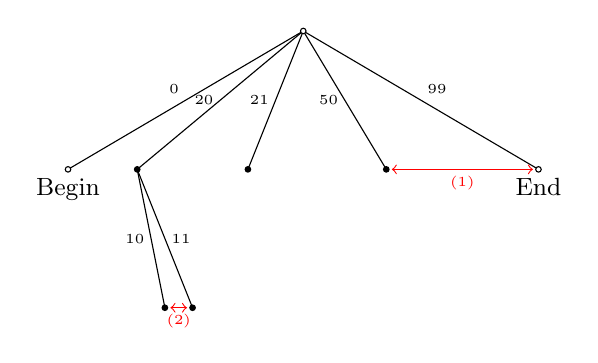
\begin{tikzpicture}[scale=1.0]
\tiny

  
  \draw (0,0) -- node[anchor=south east]{0}  (-85pt, -50pt);
  \draw (0,0) -- node[anchor=south west]{99} ( 85pt, -50pt);

  \draw (0,0) -- node[anchor=east]{20} (-60pt, -50pt);
  \draw (0,0) -- node[anchor=east]{21} (-20pt, -50pt);
  \draw (0,0) -- node[anchor=east]{50} ( 30pt, -50pt);

  \draw[fill=white] (0,0) circle (1pt);

  \draw[<->,color=red] (32pt,-50pt) -- node[anchor=north]{(1)} (83pt, -50pt);


\small
  \draw[fill=white] (-85pt, -50pt) node[anchor=north]{Begin} circle (1pt);
  \draw[fill=white] ( 85pt, -50pt) node[anchor=north]{End} circle (1pt);

\tiny
  \draw (-60pt,-50pt) -- node[anchor=east]{10} (-50pt, -100pt);
  \draw (-60pt,-50pt) -- node[anchor=west]{11} (-40pt, -100pt);

  \draw[<->,color=red] (-48pt,-100pt) -- node[anchor=north]{(2)} (-42pt,
  -100pt);

\small
  \draw[fill=black] (-60pt, -50pt) circle (1pt);
  \draw[fill=black] (-20pt, -50pt) circle (1pt);
  \draw[fill=black] ( 30pt, -50pt) circle (1pt);

  \filldraw[black](-50pt, -100pt) circle (1pt);
%  \filldraw[black] (-30.8pt, -100pt) node[anchor=north]{23} circle (1pt);
  \filldraw[black](-40pt, -100pt) circle (1pt);
%  \filldraw[black] (-12.0pt, -100pt) node[anchor=north]{70} circle (1pt);
%  \filldraw[black](- 3.2pt, -100pt) circle (1pt);


\end{tikzpicture}

\end{center}
\caption{Underlying 100-ary tree model of variable-size identifiers CRDTs. It
  contains 5 identifiers. 3 identifiers at depth-1: [20], [21], [50] and 2
  identifiers at depth-2: [20.10], [20.11]. For the sake of simplicity the
  elements linked to identifiers are not displayed.}
\label{fig:treeexample}
\end{figure}

Figure~\ref{fig:treeexample} illustrates the underlying model of variable-size
CRDTs.  If an insertion operation is performed at (1), the allocation strategy
chooses an identifier [X] with $50<X<99$. When the insert operation is
performed at (2), there is no room for another identifier, therefore, the new
identifier will be a sequence of three numbers: [20.10.X], where $0<X<100$.

These identifiers can grow linearly depending on the position of insert
operations.

Recently, LSEQ~\cite{nedelec2013lseq} lowered the space complexity of these
CRDTs from linear to sub-linear without favouring any editing behaviour. This
improvement aims to get rid of the previously mandatory garbage collecting
protocol. Three aspects define LSEQ:
\begin{itemize}
\item{base doubling:} regarding the underlying tree model, each node can have
  twice more children than its parent. It follows the properties of exponential
  trees~\cite{andersson2007dynamic}.
\item{two antagonist allocation strategies:} \emph{boundary+} and
  \emph{boundary--} that are designed for end-edition and front-edition
  respectively.
\item{random strategy choice:} it randomly assigns an allocation strategy to
  each depth of the tree. It follows the intuition: \emph{since we have no
    prior knowledge of the editing behaviour, the strategy choice should not
    favor any editing behaviour. Consequently, the frequencies of appearance of
    each allocation strategy have to be equal.}
\end{itemize}

Despite the fact that numerous experiments have been performed using LSEQ
including real documents extracted from Wikipedia, they did not include any
concurrency. Although, Wikipedia's revisions already present a serialization of
the document without explicit concurrency, experiments with this type of
documents are of great importance~\cite{ahmed2011evaluating}.

\begin{table}[h]
  \begin{center}
    \begin{tabular}{|l|r|r|r|r|r|}
      \cline{2-6}
      \multicolumn{1}{c|}{} & \multicolumn{5}{c|}{\textbf{\#insert operations}}
      \\
      %%\cline{2-6}
      \multicolumn{1}{c|}{} & \textbf{10} & \textbf{100} & \textbf{200}
      & \textbf{500} & \textbf{1000} \\
      \hline
      1 user (bit/id) & 6.5 & 26.8 & 32.7 & 56.0 & 64.2 \\
      \hline
      10 users (bit/id) & 9.5 & 125.8 & 377.0 & 1962.1 & 5468.0 \\
      \hline
    \end{tabular}
    \caption{Average bit-length of LSEQ identifiers for single and multiple
      user(s) and the generation of documents of 10, 100, 200, 500, and 1000
      lines.}
    \label{tab:motivating}
  \end{center}
\end{table} 

Table~\ref{tab:motivating} shows the average bit-length of the identifiers
assigned by LSEQ on different size synthetic documents created either by a
single user or by a group of 10 collaborators. Both documents were edited at
the end. We observe that while the identifiers resulting from a single author
are sub-linearly upper-bounded, the bit-length of identifiers generated by 10
users are quadratically increasing.

\begin{Def}[Problem statement]
  Let $\mathcal{D}$ be a document on which n insert operations have been
  performed. Let $\mathcal{I}(\mathcal{D}) = \{id|(\_, id) \in
  \mathcal{D}\}$. The function alloc($id_p$,$id_q$) should provide identifiers
  such as:
  \begin{center}
    $\sum\limits_{id \in \mathcal{I}} {{ log_2(id)}\over{n}} $ $< O(n)$
  \end{center}
\label{def:problem}
\end{Def}

Definition~\ref{def:problem} from~\cite{nedelec2013lseq} states the $alloc$
function property: a sub-linear upper-bound on the average bit-length of
identifiers. By excluding any reference to the two phases of optimistic
replication operations, it encompasses both the local generation of identifiers
and the integration of remote operations.  According to
Table~\ref{tab:motivating}, LSEQ only partially answers the problem statement.


The identified problem concerns the preservation of the space complexity of
LSEQ from single user to multiple users edition. Using multiple antagonist
strategies without any coordination between collaborators leads to a quadratic
growth of identifiers. Consequently, providing a mechanism of agreement in the
choice of strategies would greatly improve LSEQ as well as any composition of
allocation strategies. Furthermore, such improvement would make variable-size
identifiers CRDTs actually usable in the distributed collaborative editing
context.

%%% Local Variables: 
%%% mode: latex
%%% TeX-master: "../dchanges"
%%% End: 
